\documentclass[11pt,a4paper]{article}
\usepackage[utf8]{inputenc}
\usepackage[T1]{fontenc}
\usepackage{amsthm} %numéroter les questions
\usepackage[english]{babel}
\usepackage{datetime}
\usepackage{xspace} % typographie IN
\usepackage{hyperref}% hyperliens
\usepackage[all]{hypcap} %lien pointe en haut des figures
\usepackage[french]{varioref} %voir x p y
\usepackage{fancyhdr}% en têtes
%\input cyracc.def
\usepackage[]{graphicx} %include pictures
\usepackage{pgfplots}
\usepackage[]{circuitikz}
\usepackage{ifthen}

\usepackage[top=1.3 in, bottom=1.3 in, left=1.3 in, right=1.3 in]{geometry} % Yeah, that's bad to play with margins
\usepackage[]{pdfpages}

\usepackage[]{attachfile}

\usepackage{float}
\usepackage{subfig}

\usepackage{todonotes} % \missingfigure
\usepackage{gensymb} % \ohm

\usepackage{framed}
\usepackage[many]{tcolorbox}

\newdateformat{mydate}{v2.0.0}%hack pour remplacer \THEYEAR


\newboolean{corrige}
\ifx\correction\undefined
\setboolean{corrige}{false}% pas de corrigé
\else
\setboolean{corrige}{true}%corrigé
\fi

%\setboolean{corrige}{false}% pas de corrigé

\newboolean{annexes}
\setboolean{annexes}{true}%annexes
%\setboolean{annexes}{false}% pas de annexes

\definecolor{darkblue}{rgb}{0,0,0.5}

\newboolean{mos}
%\setboolean{mos}{true}%annexes
\setboolean{mos}{false}% pas de annexes

\usepackage{aeguill} %guillemets

%% fancy header & foot
\pagestyle{fancy}
%Numero du TP :
\def \labonumber {Project -- Part 2}
\lhead{[ELEC-H-310] Digital electronics\\ \labonumber}
\rhead{\mydate\today\\ page \thepage}
\chead{\ifthenelse{\boolean{corrige}}{Corrigé}{}}
\cfoot{}
%%

\pdfinfo{
/Author (ULB -- BEAMS)
/Title (\labonumber ELEC-H-310)
/ModDate (D:\pdfdate)
}

\hypersetup{
pdftitle={\labonumber [ELEC-H-310] Choucroute numérique},
pdfauthor={ULB -- BEAMS},
pdfsubject={}
}

\theoremstyle{definition}% questions pas en italique
\newtheorem{Q}{Question}[] % numéroter les questions [section] ou non []

\newcommand{\reponse}[1]{% pour intégrer une réponse : \reponse{texte} : sera inclus si \boolean{corrige}
	\ifthenelse {\boolean{corrige}} {\paragraph{Réponse :} \color{darkblue}   #1\color{black}} {}
 }

\newcommand{\addcontentslinenono}[4]{\addtocontents{#1}{\protect\contentsline{#2}{#3}{#4}{}}}

\date{\vspace{-1.7cm}\mydate\today}
\title{\vspace{-2cm}\labonumber \\ Digital electronics [ELEC-H-310]\\Design of an automatic fanning system: \\ Luminous intensity acquisition and fan control\ifthenelse{\boolean{corrige}}{~\\Corrigé}{}}

\setlength{\parskip}{0.2cm plus2mm minus1mm} %espacement entre §
\setlength{\parindent}{0pt}


















\begin{document}
% \pagestyle{empty}
\maketitle
% \vspace*{-1cm}




% ########   ##     ##  ##########  
% ##     ##  ##     ##      ##      
% ##     ##  ##     ##      ##      
% ########   ##     ##      ##      
% ##     ##  ##     ##      ##      
% ##     ##  ##     ##      ##      
% ########    #######       ##      

\section*{Aims}
During three laboratory sessions, you will have to design a small automatic fanning system based on a propeller fan.
During the second lab session, you will implement an open-loop fan control based on luminous intensity.

\section*{Prerequisite}
Before entering in the lab, you have to read the project specifications defined in the document ``Design of an automatic fanning system".


\section*{Objectives}
At the end of this lab session, you'll be able to:
\begin{itemize}
	\item Size a data acquisition system for $\mu$C.
	\item Design and implement a simple control system.
\end{itemize}


\newpage




% ########   ##      ##  ##########  ########     #####    
%    ##      ###     ##      ##      ##     ##  ##     ##  
%    ##      ## ##   ##      ##      ##     ##  ##     ##  
%    ##      ##  ##  ##      ##      ########   ##     ##  
%    ##      ##   ## ##      ##      ##   ##    ##     ##  
%    ##      ##     ###      ##      ##    ##   ##     ##  
% ########   ##      ##      ##      ##     ##    #####    


\section{Introduction}
During three laboratory sessions, you will have to design an automatic fanning system based on a propeller fan.

During this second lab, your first aim will be to measure the luminous intensity of the environment.
In order to do this, you have to design a data acquisition system allowing to acquire a voltage representing the luminous intensity.

On the basis of this measure, you will design a controller that will adapt the propeller speed.






%    ###      #######     #####    ##     ##  ########    #######   ########   ##########  ########     #####    ##      ##  
%   ## ##    ##     ##  ##     ##  ##     ##     ##      ##     ##     ##          ##         ##      ##     ##  ###     ##  
%  ##   ##   ##         ##     ##  ##     ##     ##      ##            ##          ##         ##      ##     ##  ## ##   ##  
% ##     ##  ##         ##     ##  ##     ##     ##       #######      ##          ##         ##      ##     ##  ##  ##  ##  
% #########  ##         ##    # #  ##     ##     ##             ##     ##          ##         ##      ##     ##  ##   ## ##  
% ##     ##  ##     ##    #### #   ##     ##     ##      ##     ##     ##          ##         ##      ##     ##  ##     ###  
% ##     ##   #######           #   #######   ########    #######   ########       ##      ########     #####    ##      ##  



\section{Design of the data acquisition system}

\begin{figure}[H]
\center
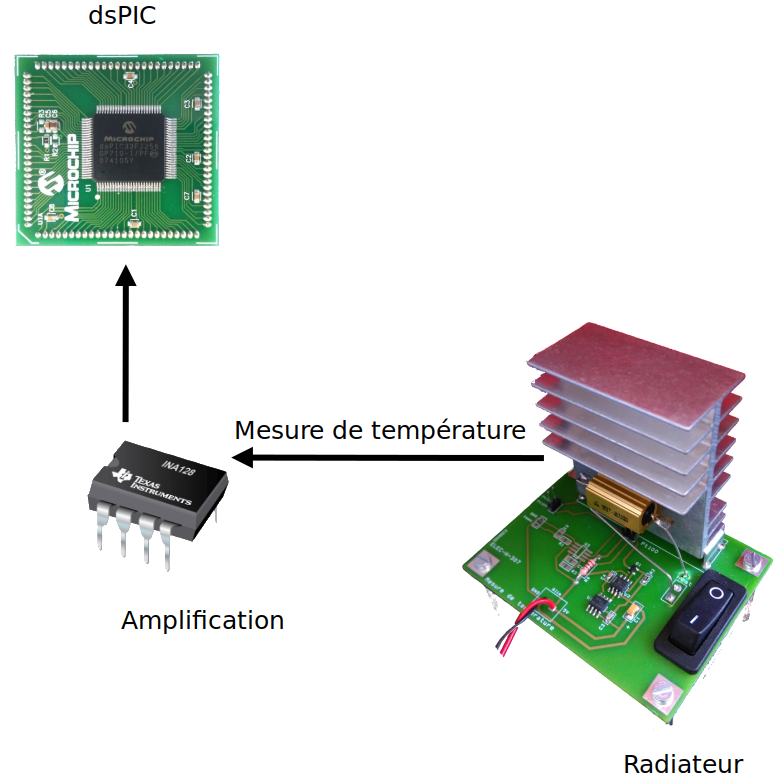
\includegraphics[width=0.8\textwidth]{acquisition}
\caption{illuminance acquisition chain.}
\label{fig:acquisition}
\end{figure}

As explained in the project specifications, the measure of the luminous intensity is realized by measuring a voltage over a voltage divider. In order to have a measurement that fits within the range of the ADC, you will need to choose the value of the fixed resistor appropriately. 


\tcboxfit[height=5.5cm,title={Voltage divider.},
  before=\noindent]{%
  \begin{minipage}{.2\linewidth}
  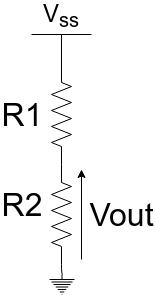
\includegraphics[height=4cm]{voltage_divider.png}
  \end{minipage}
  \begin{minipage}{.78\linewidth}
  Let's express $V_{out}$ using $R_1$, $R_2$ and $V_{ss}$.
  Assuming $V_{ss}$ delivers a current $i$, Kirchhoff tells us that $V_{ss} - R_1 \cdot i - R_2 \cdot i = 0$.
  Moreover, using Ohm's law we have $V_{out} = R_2 \cdot i \Leftrightarrow i = \frac{V_{out}}{R_2}$.
  Injecting this last expression into the first one yields $V_{ss} - R_1 \cdot \frac{V_{out}}{R_2} - R_2 \cdot \frac{V_{out}}{R_2} = 0$, from which we can find \[ V_{out} = \frac{R_2}{R_1 + R_2}\cdot V_{ss} \]
  This last relation is the canonical expression of a voltage divider.
  \end{minipage}
}


This measurement, if designed appropriately, can be digitized directly by the PSOC system (see figure~\ref{fig:acquisition}).

\begin{itemize}
	\item The illuminance in indoor environments can vary from 1 (pitch black) to 10000 (bright indoors). However, the variability of photoresistor manufacturing can be quite big. Use the ohmmeter to measure the value of the photoresistor under different lighting conditions. 
	\item Given the possible range of photoresistor values, choose the other resistor of the voltage divider appropriately to exploit the range of the ADC as much as possible. 
	\item As the analog-to-digital converter digitizes the voltage on 16 bits and is supplied with 5V, what is its resolution?
	\item Given the values you chose for the resistor, what is the minimum and maximum voltage you expect to measure at the ADC? 
\end{itemize}

Now, we will design and implement the data acquisition system.
\begin{itemize}
	\item Connect the circuit on your protoboard and check if it works by measuring the signal with a voltmeter.
	\item Connect the voltage to be digitized to the input of your PSOC ADC through one of the GPIOs J1 or J2. 
\end{itemize}






%  #######     #####    ##      ##  #########  ########    #######   ##     ##  ########      ###     ##########  ########     #####    ##      ##  
% ##     ##  ##     ##  ###     ##  ##            ##      ##         ##     ##  ##     ##    ## ##        ##         ##      ##     ##  ###     ##  
% ##         ##     ##  ## ##   ##  ##            ##      ##         ##     ##  ##     ##   ##   ##       ##         ##      ##     ##  ## ##   ##  
% ##         ##     ##  ##  ##  ##  ######        ##      ##   ####  ##     ##  ########   ##     ##      ##         ##      ##     ##  ##  ##  ##  
% ##         ##     ##  ##   ## ##  ##            ##      ##     ##  ##     ##  ##   ##    #########      ##         ##      ##     ##  ##   ## ##  
% ##     ##  ##     ##  ##     ###  ##            ##      ##     ##  ##     ##  ##    ##   ##     ##      ##         ##      ##     ##  ##     ###  
%  #######     #####    ##      ##  ##         ########   ########    #######   ##     ##  ##     ##      ##      ########     #####    ##      ##  



\section{Configuration of the analog-to-digital converter}
Now, you will program the analog-to-digital converter so that you obtain a ``digital image" of the illuminance.
\begin{itemize}
	\item Instantiate an ADC in your topDesign.cysch file, and adapt the firmware (i.e. the main.c) to read the values from the ADC. You can do this either through polling or through ISRs. The illuminance should be digitized every 0.5~ms. 
	\item Instantiate a ``Character LCD" in your topDesign.cysch file. Connect the LCD inputs using the ``Extension PSOC" file. 
	\item By using the API described in the datasheet of the LCD, write something on the LCD screen. Note that the 8 first characters of the LCD screen are defined to be row~1, the 8 last characters of the LCD screen are defined to be row~2. 
	\item Based on your data acquisition system, write the value of the measured voltage on the LCD screen in the format ``Vr=2.41". There should be two digits after the comma. The LCD refresh rate should be 1~Hz. 
\end{itemize}






% ########   #########   #######   ##     ##  ##            ###     ##########  ########     #####    ##      ##  
% ##     ##  ##         ##         ##     ##  ##           ## ##        ##         ##      ##     ##  ###     ##  
% ##     ##  ##         ##         ##     ##  ##          ##   ##       ##         ##      ##     ##  ## ##   ##  
% ########   ######     ##   ####  ##     ##  ##         ##     ##      ##         ##      ##     ##  ##  ##  ##  
% ##   ##    ##         ##     ##  ##     ##  ##         #########      ##         ##      ##     ##  ##   ## ##  
% ##    ##   ##         ##     ##  ##     ##  ##         ##     ##      ##         ##      ##     ##  ##     ###  
% ##     ##  #########  ########    #######   #########  ##     ##      ##      ########     #####    ##      ##  



\section{Speed control}
You have now all the elements to build your automatic fanning control system.
The only item missing is an open-loop controller. 

\begin{itemize}
	\item Write a function taking as an argument the illumination value.
	This control function will have to adjust the rotation speed of the propeller fan, so that it follows illuminance.
	The choice of the controller is up to you, but it does not need to be particularly complex.
	\item Check if your system works.
\end{itemize}



\end{document}
